\section{Case Study: Playing Atari Games}
\begin{frame}{}
    \LARGE Case Study: \textbf{Playing Atari Games}
\end{frame}

\begin{frame}{Case Study: Playing Atari Games}
\begin{figure}
\centering
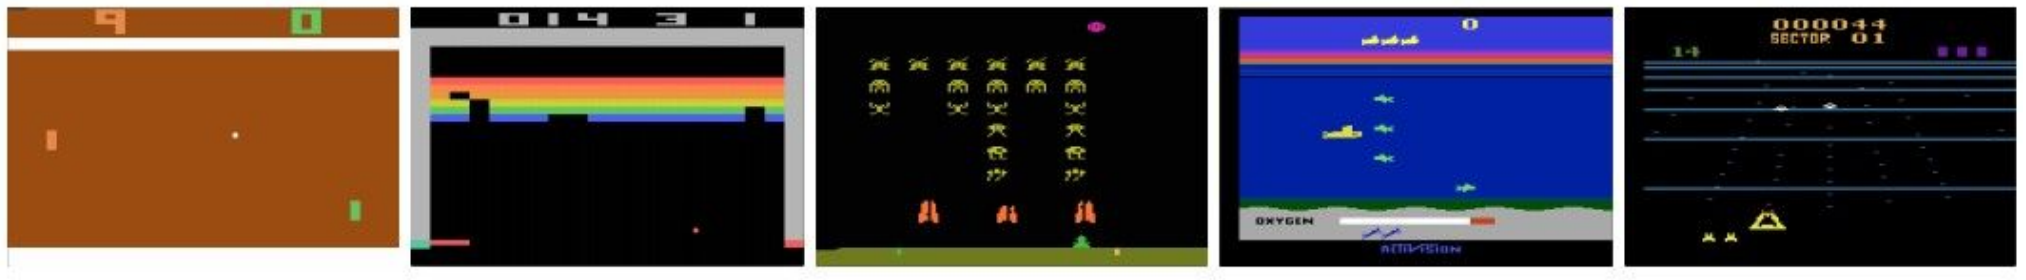
\includegraphics[width=0.9\textwidth,height=0.9\textheight,keepaspectratio]{images/dqn+sarsa/atari_1.png}
\end{figure}

\begin{itemize}
    \item \textbf{Objective}: Complete the game with the highest score
    \item \textbf{State}: Raw pixel inputs of the game state
    \item \textbf{Action}: Game controls e.g. Left, Right, Up, Down
    \item \textbf{Reward}: Score increase/decrease at each time step
\end{itemize}
\footnotetext{[Mnih et al. NIPS Workshop 2013; Nature 2015]}

\end{frame}

\begin{frame}{Case Study: Playing Atari Games}

\begin{figure}
\centering
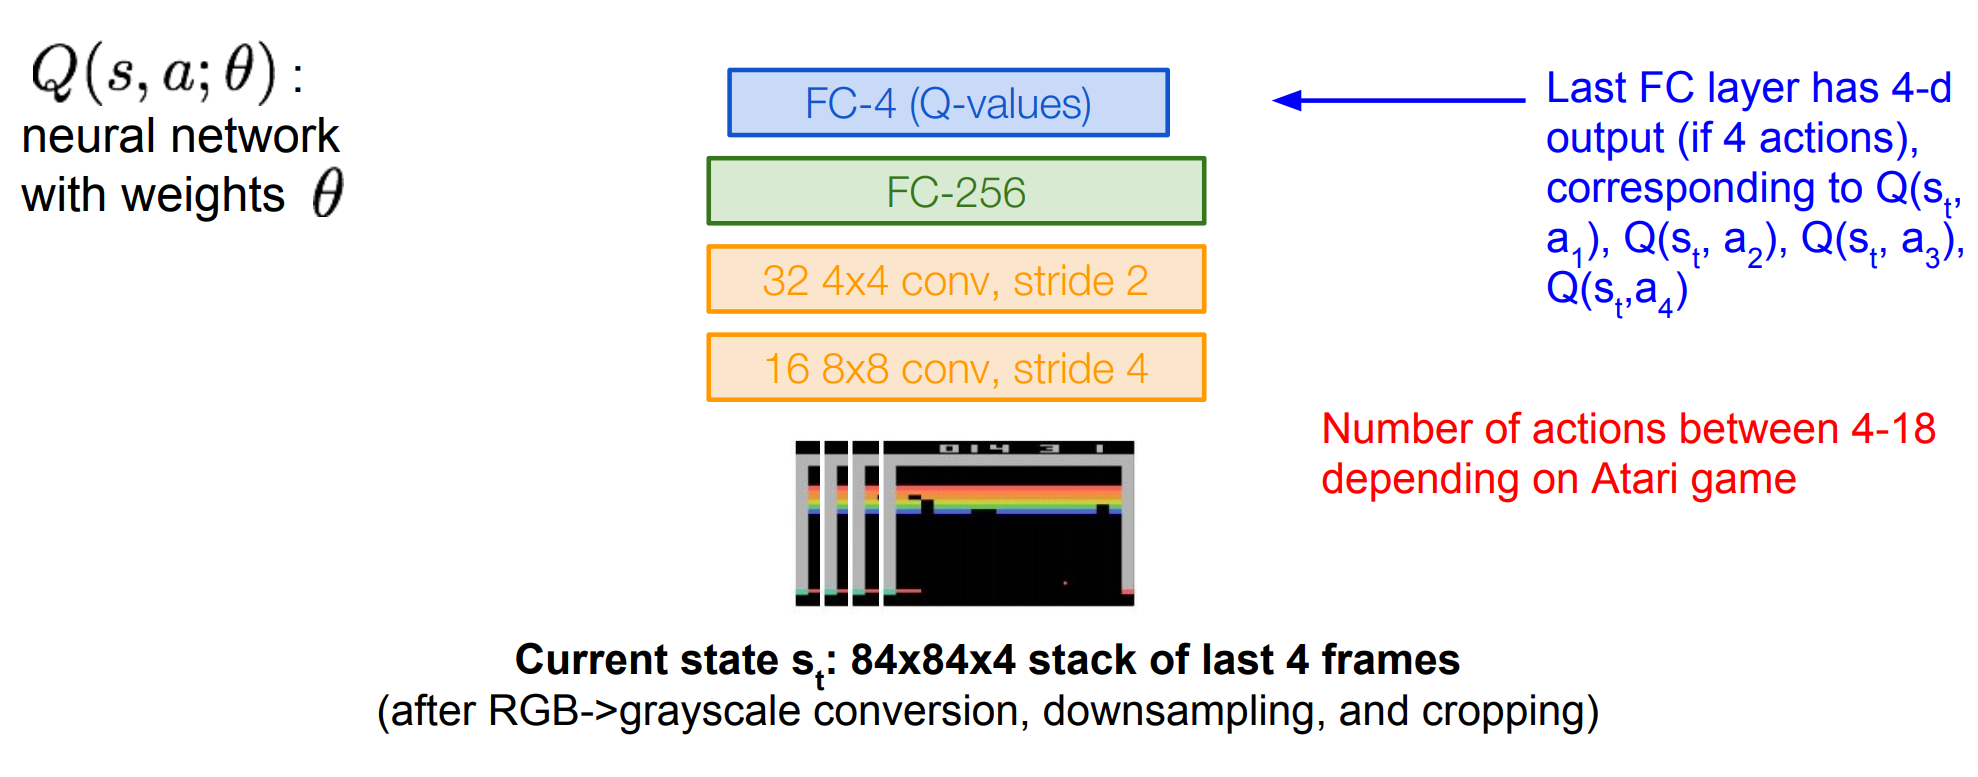
\includegraphics[width=1.0\textwidth,height=1.0\textheight,keepaspectratio]{images/dqn+sarsa/atari_2.png}
\end{figure}
\pause
\centering
\href{https://www.youtube.com/watch?v=V1eYniJ0Rnk}{https://www.youtube.com/watch?v=V1eYniJ0Rnk}

\footnotetext{[Mnih et al. NIPS Workshop 2013; Nature 2015]}
\end{frame}